\chapter{Bilag}\label{ch:bilag}

%Insert figures
\begin{figure}
    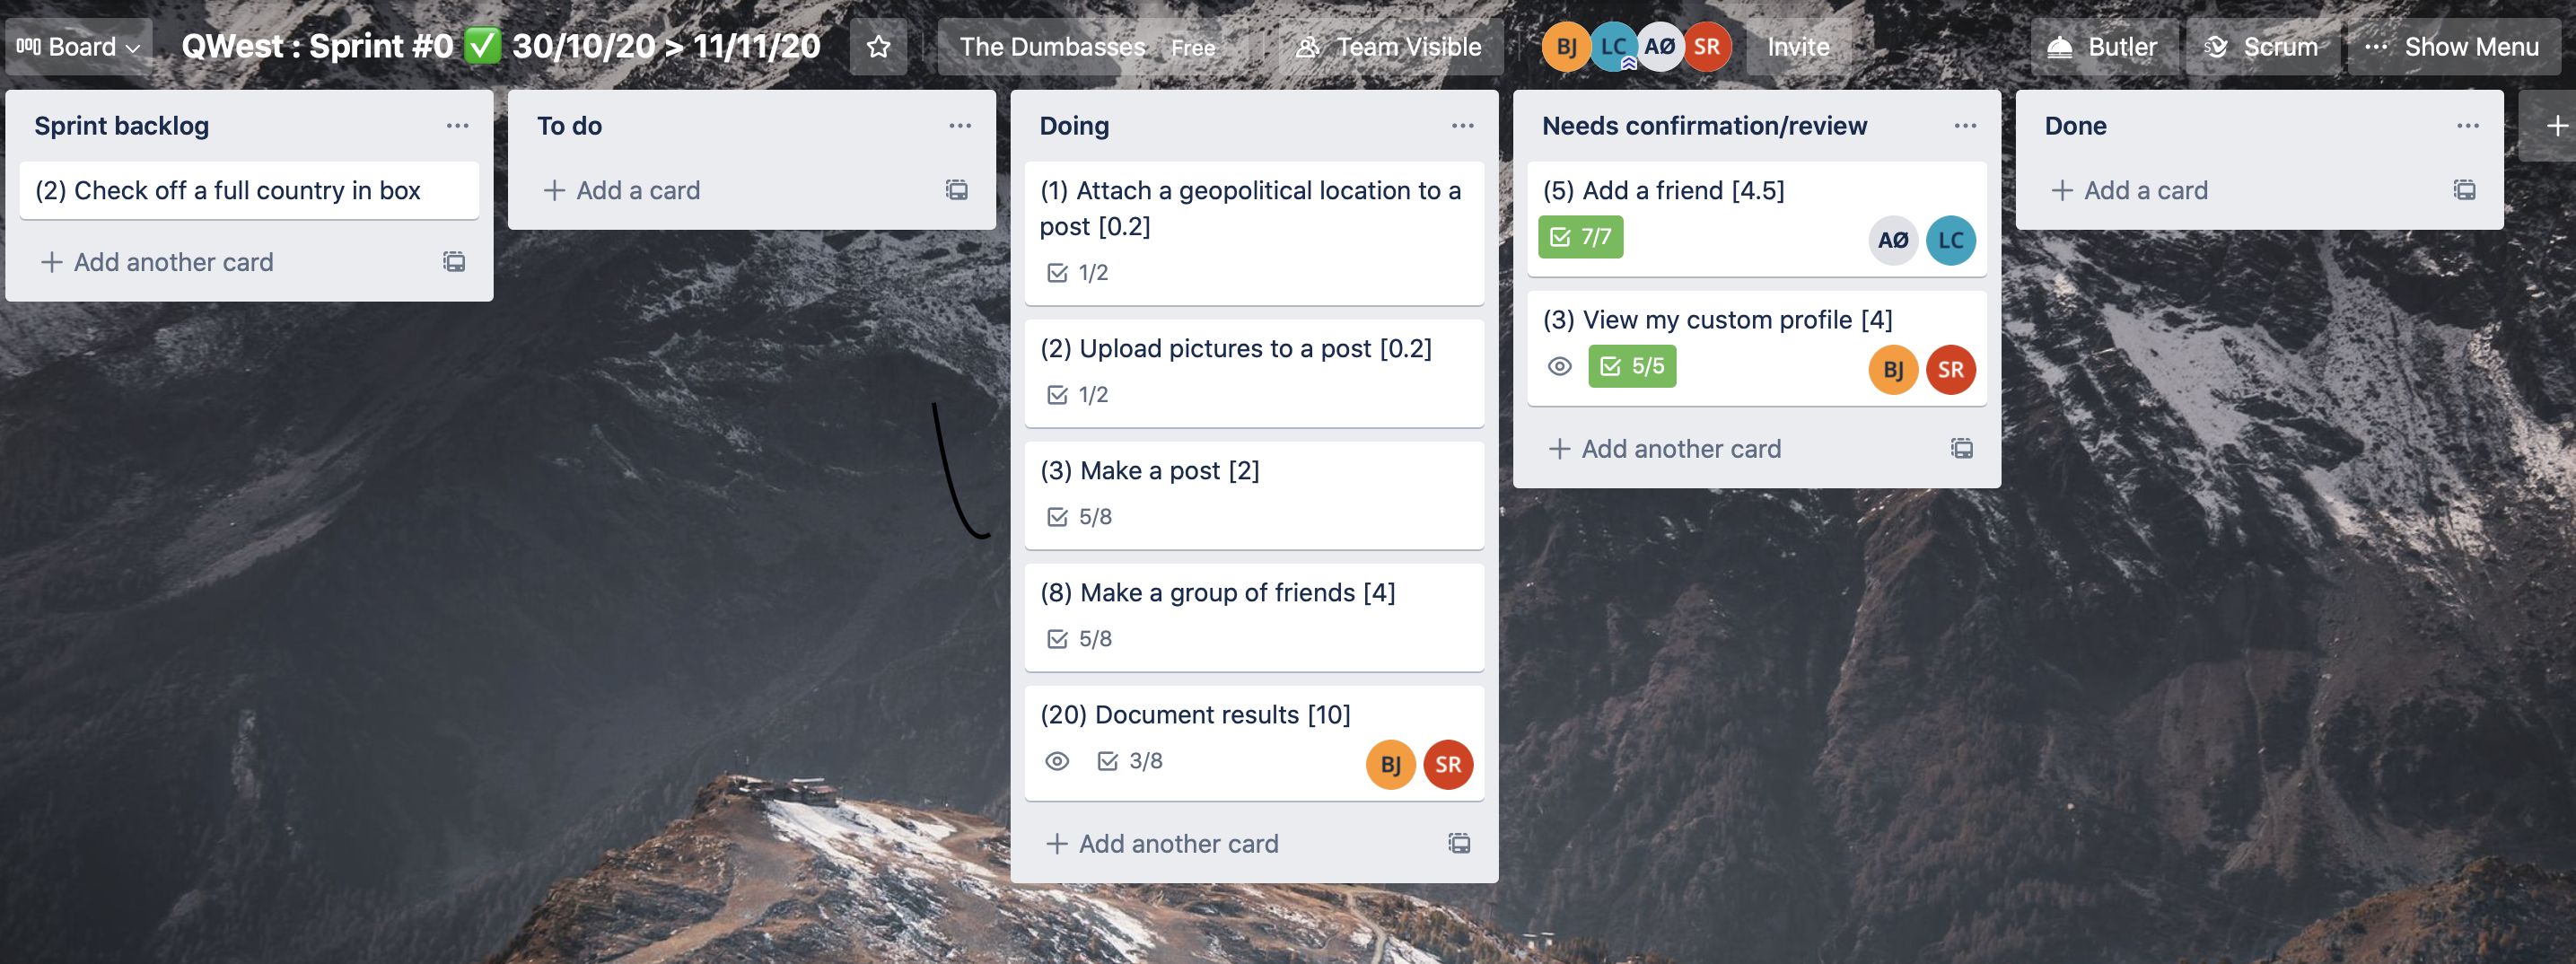
\includegraphics[width=\linewidth]{figures/Sprint 0.png}
    \caption{Sprint 0}
    \label{fig:Sp0}
\end{figure}


\begin{figure}
    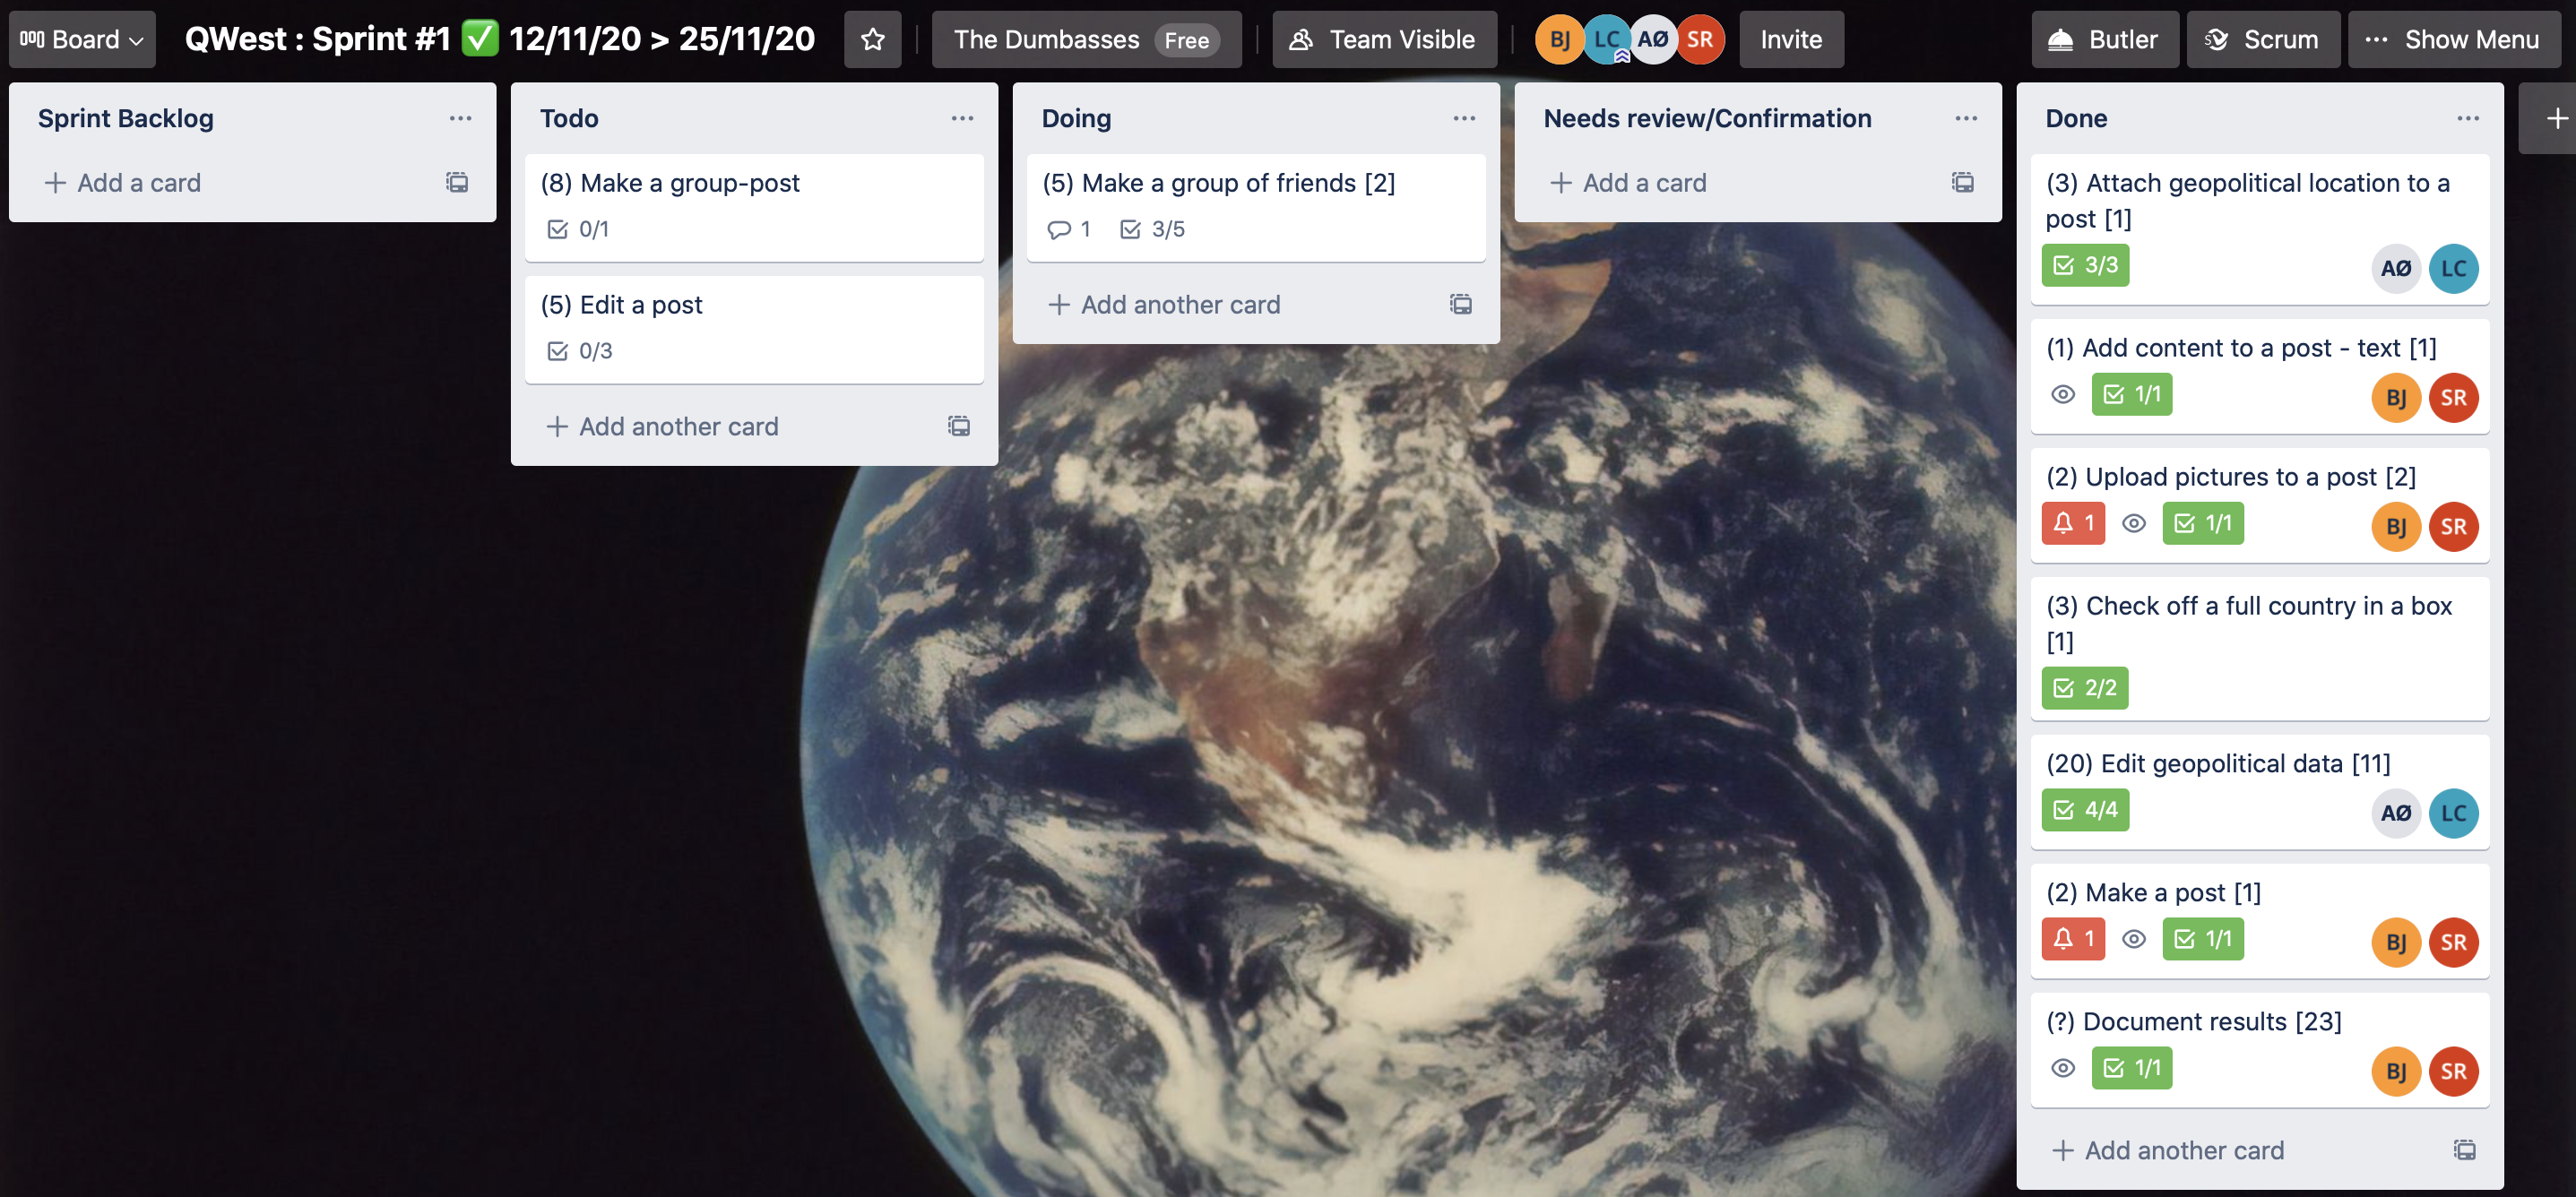
\includegraphics[width=\linewidth]{figures/Sprint 1.png}
    \caption{Sprint 1}
    \label{fig:Sp1}
\end{figure}


\begin{figure}
    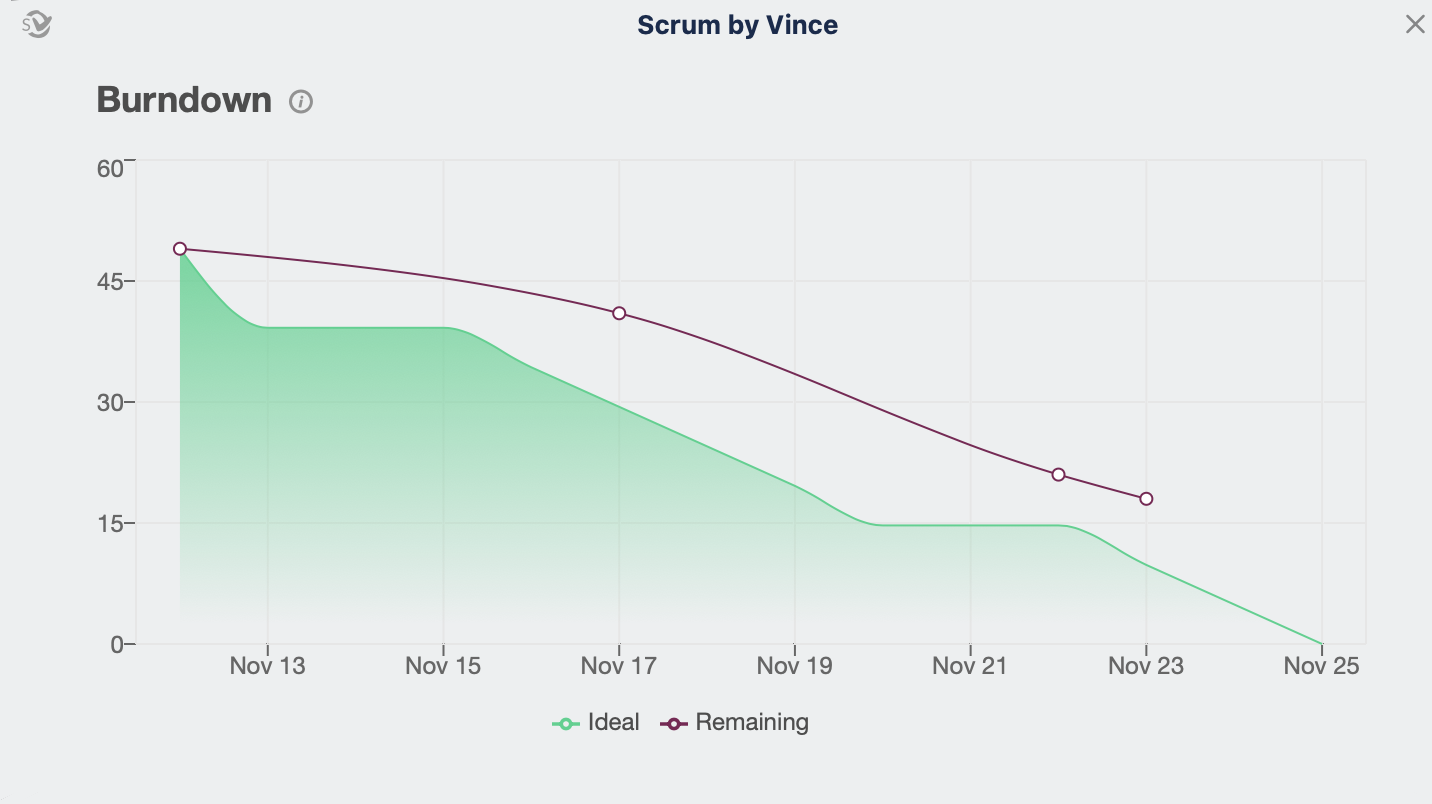
\includegraphics[width=\linewidth]{figures/Sprint 1 Burndown.png}
    \caption{Burndown chart Sprint 1}
    \label{fig:Bc1}
\end{figure}



\begin{figure}
    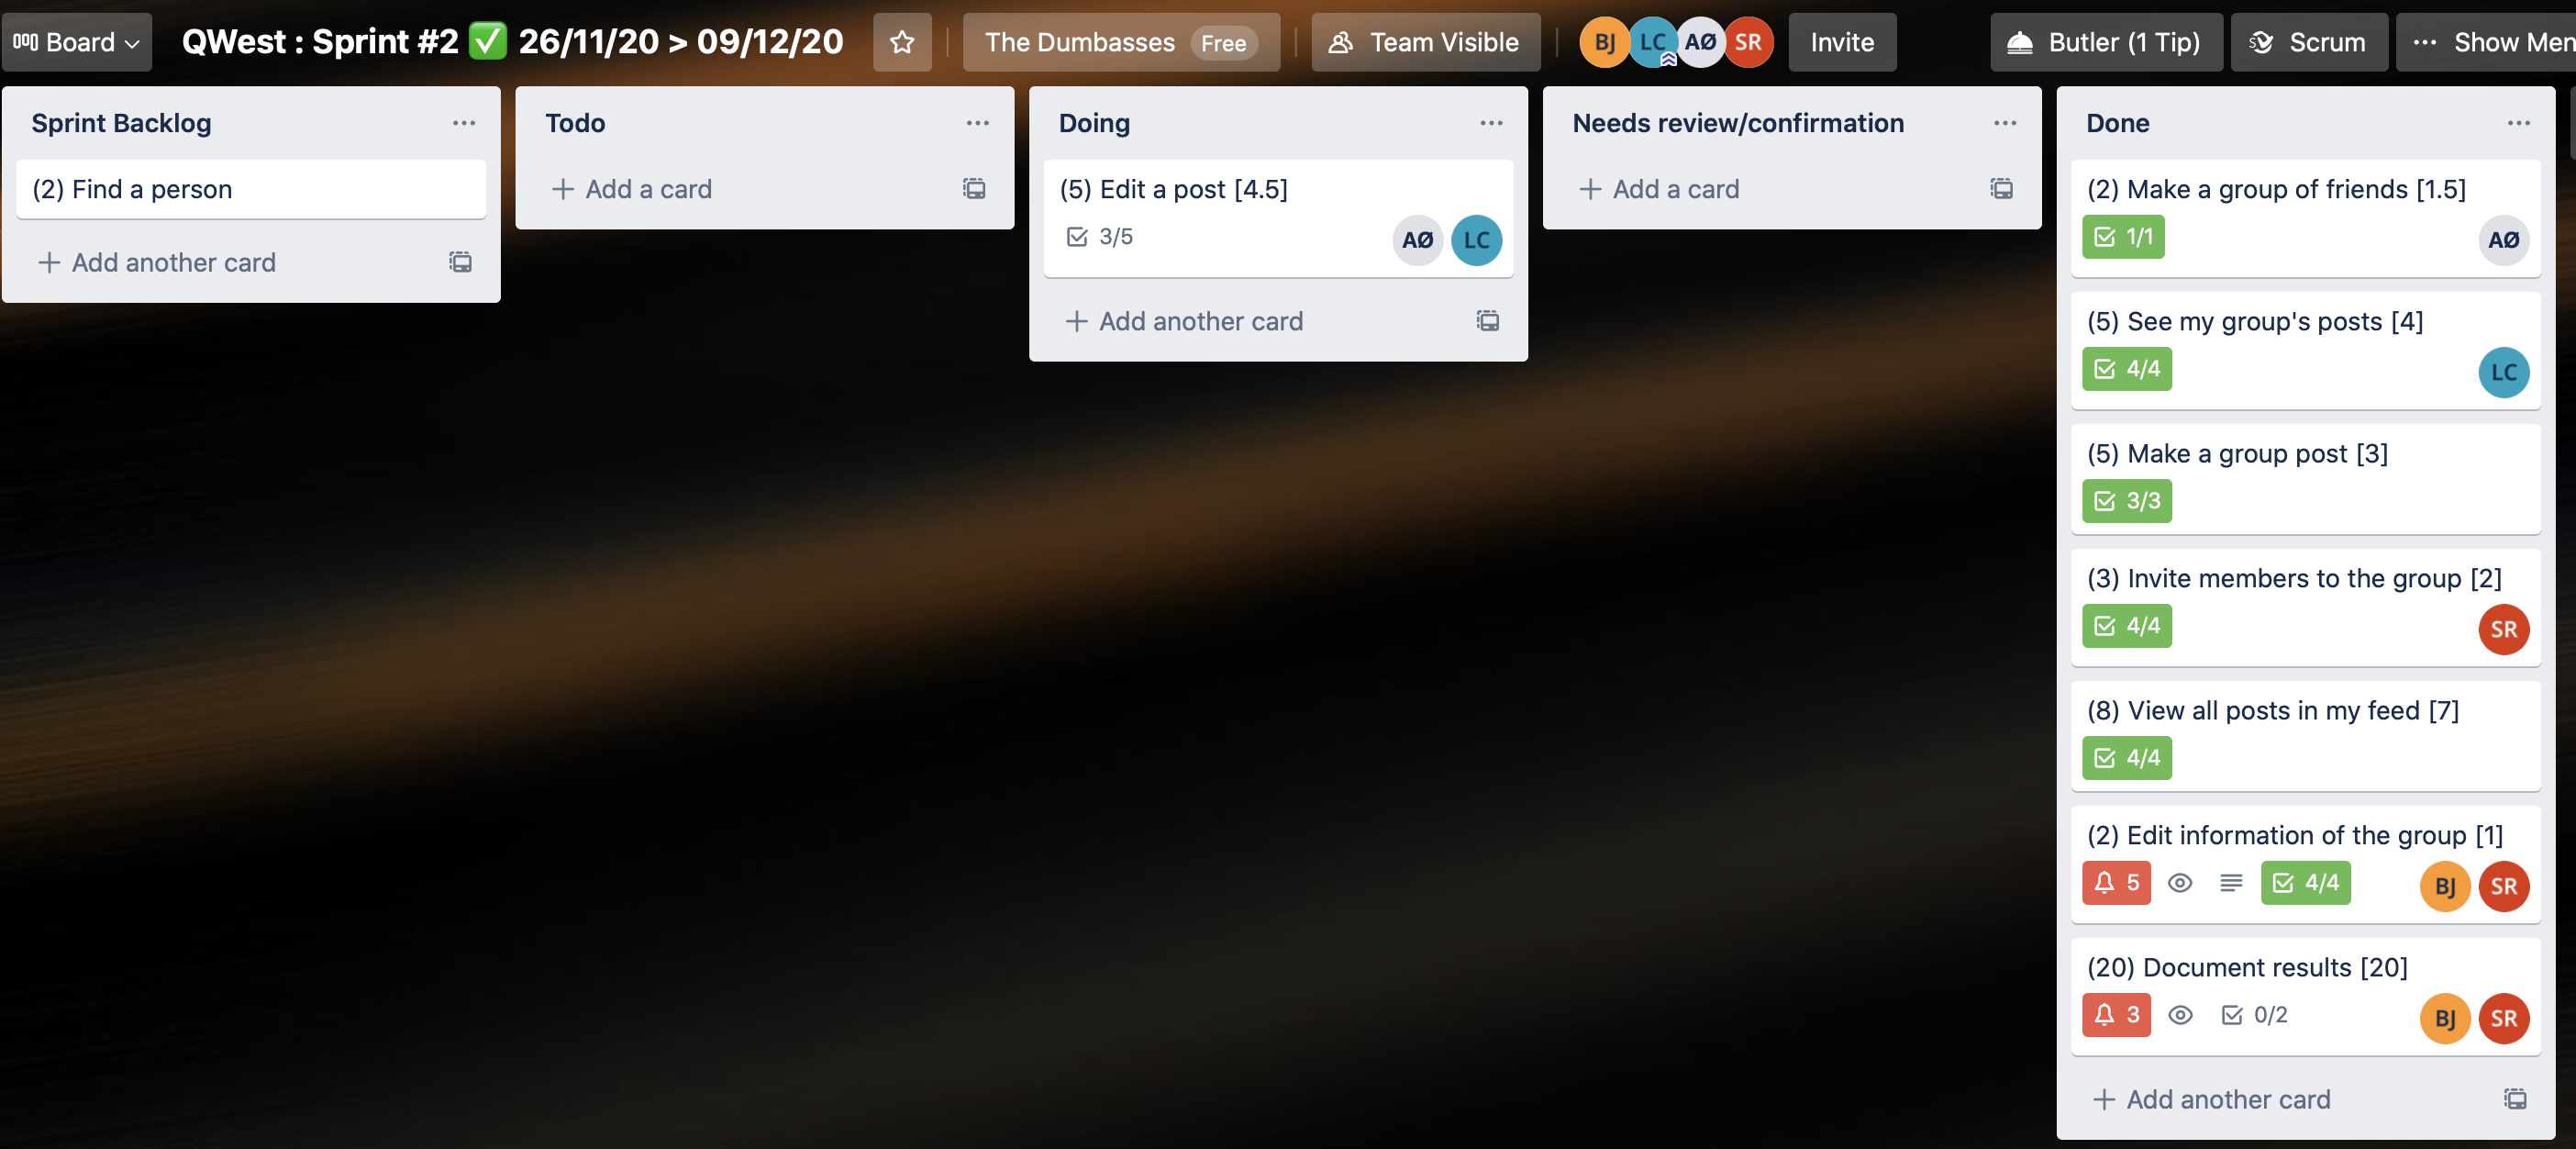
\includegraphics[width=\linewidth]{figures/Sprint 2.png}
    \caption{Sprint 2}
    \label{fig:Sp2}
\end{figure}



\begin{figure}
    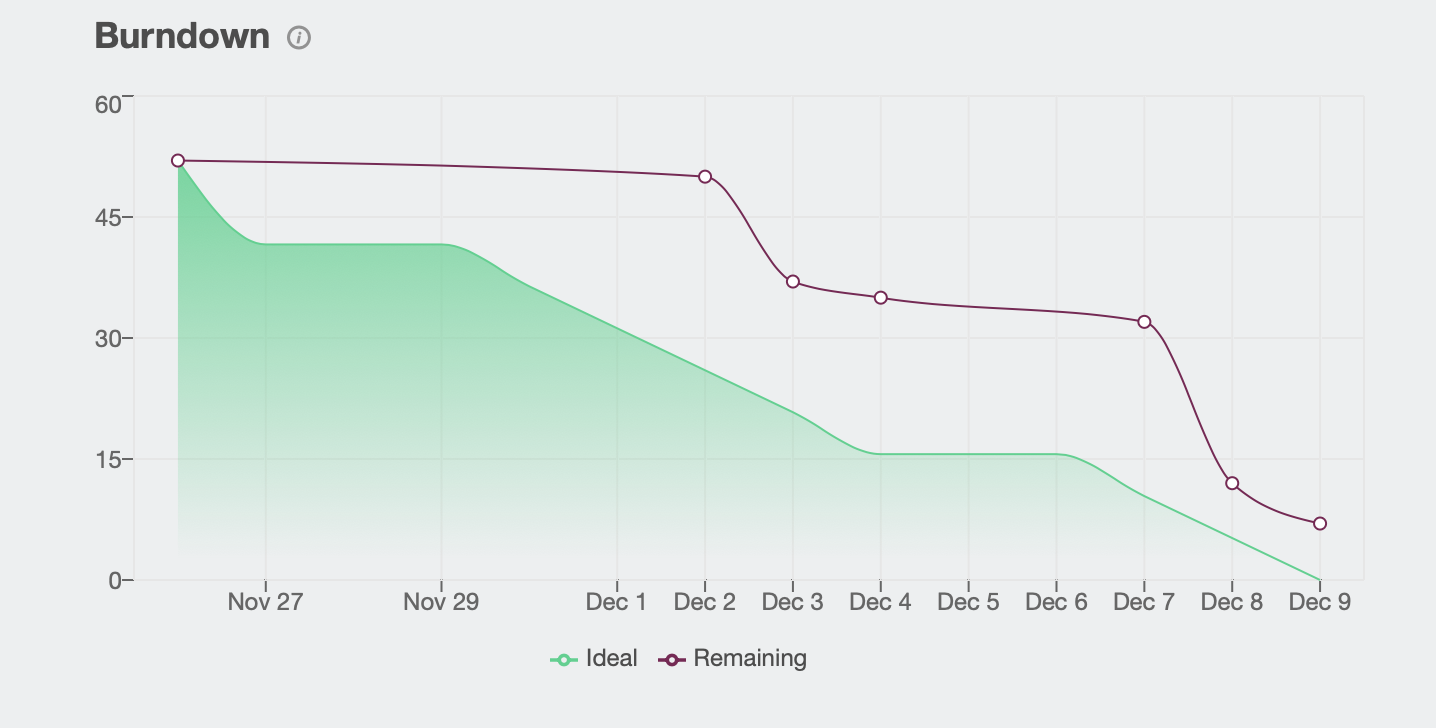
\includegraphics[width=\linewidth]{figures/Sprint 2 Burndown.png}
    \caption{Burndown Chart Sprint 2}
    \label{fig:Bc2}
\end{figure}

\begin{figure}
    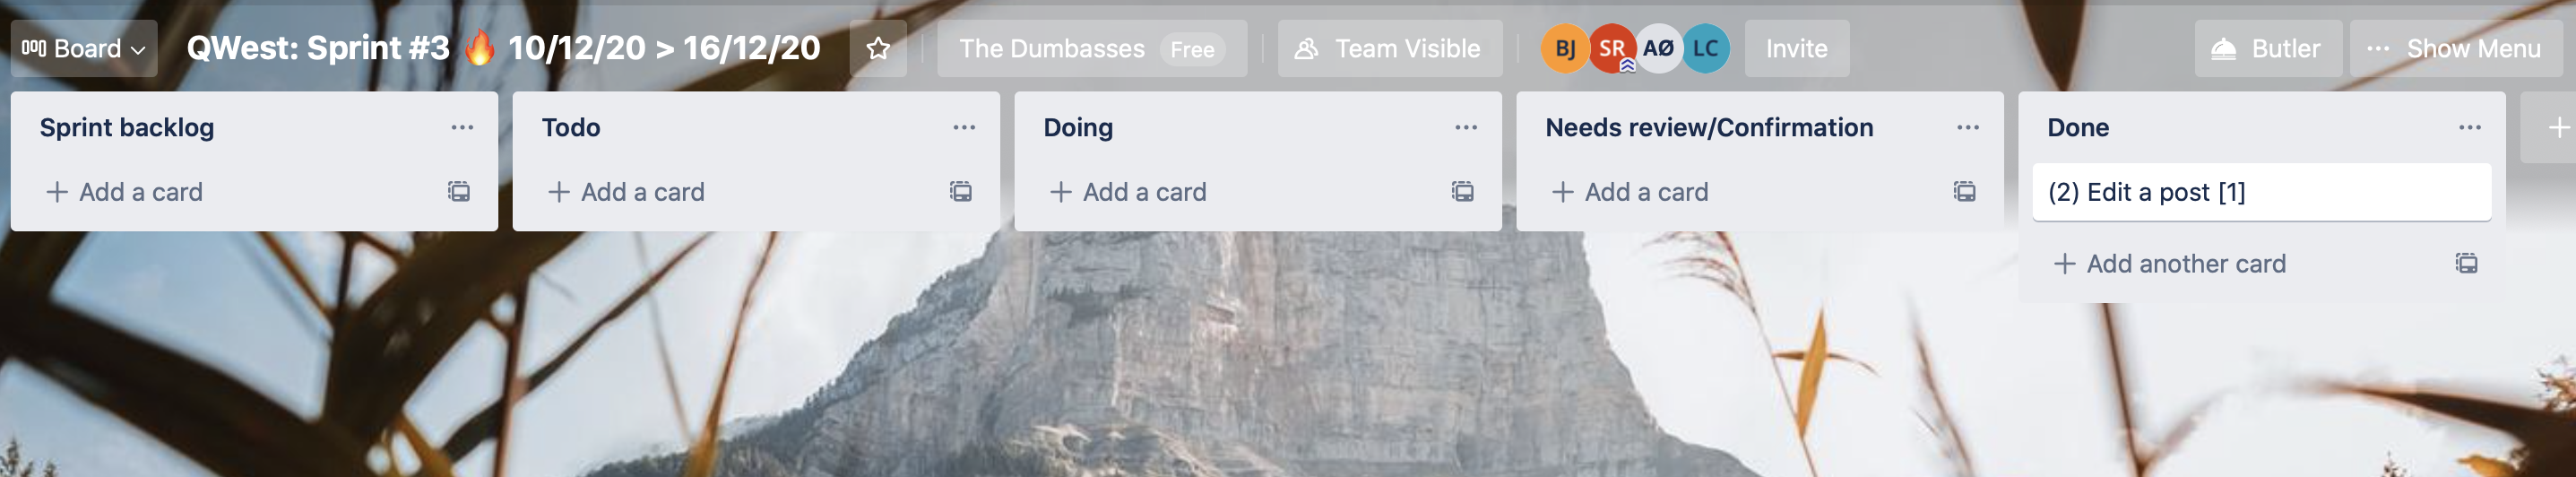
\includegraphics[width=\linewidth]{figures/Sprint 3 .png}
    \caption{{Sprint 3}}
    \label{fig:Sp3}
\end{figure}


\begin{figure}
    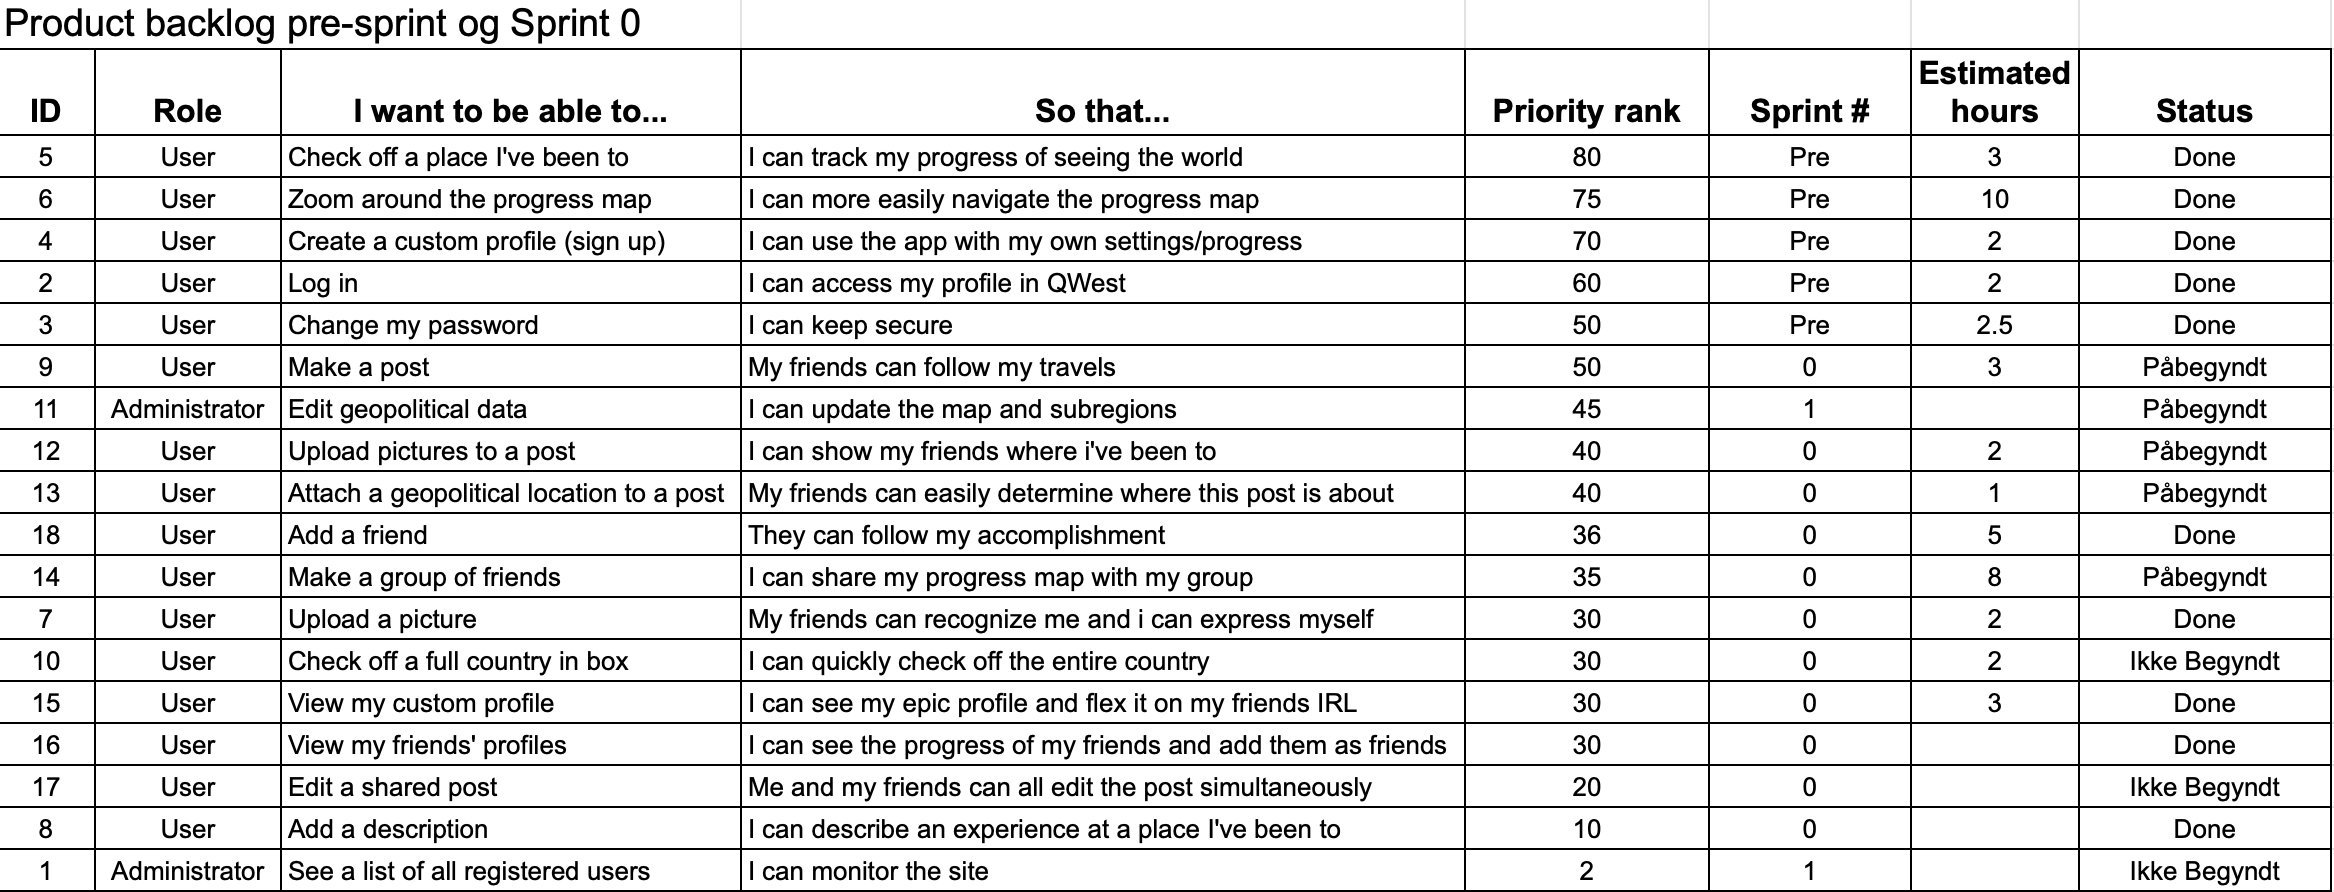
\includegraphics[width=\linewidth]{figures/Sprint 0 copy.png}
    \caption{{Sprint 0 Produkt Backlog}}
    \label{fig:Sp0PB}
\end{figure}


\begin{figure}
    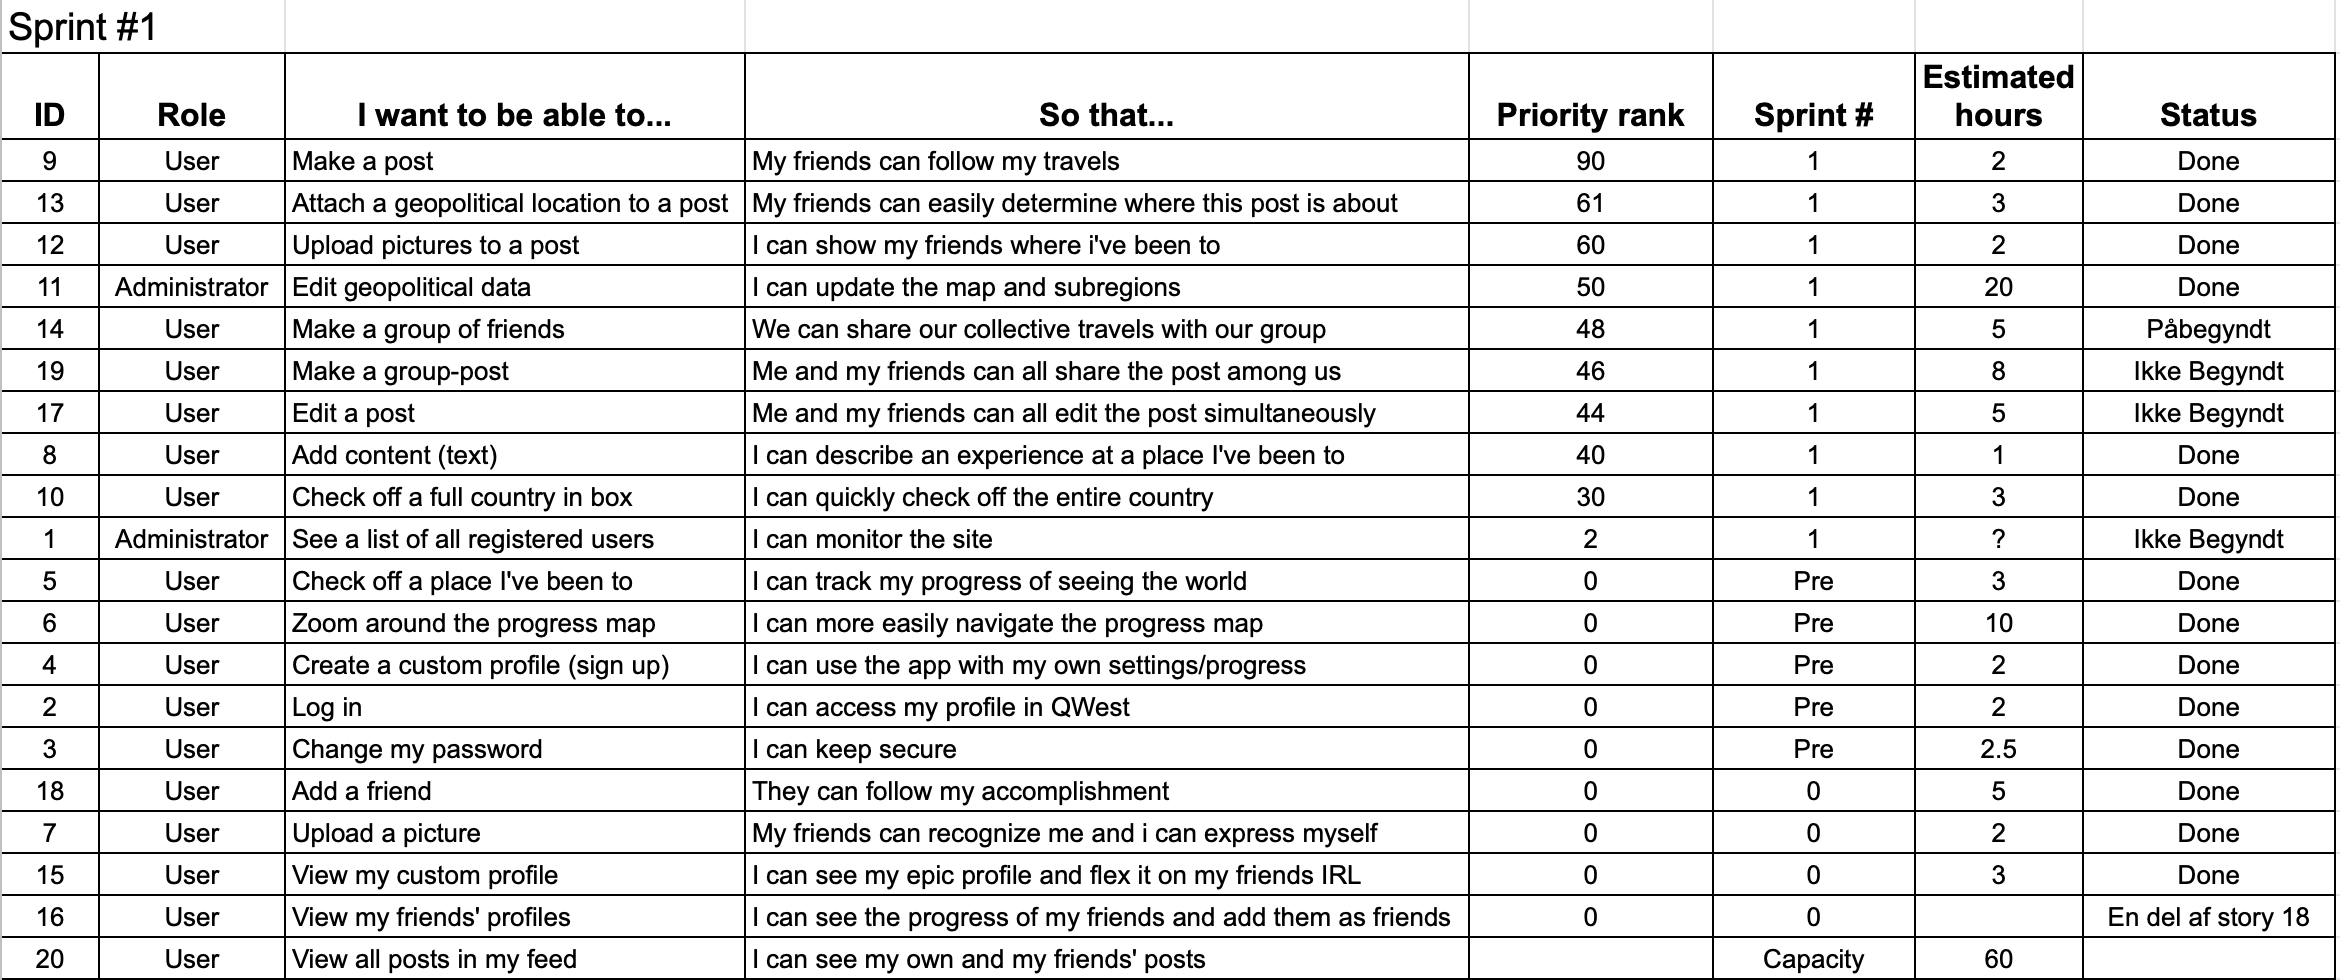
\includegraphics[width=\linewidth]{figures/Sprint 1 copy.png}
    \caption{{Sprint 1 Produkt Backlog}}
    \label{fig:Sp1PB}
\end{figure}


\begin{figure}
    \includegraphics[width=\linewidth]{figures/Sprint 2 copy.png
    \caption{{Sprint 2 Produkt Backlog}}
    \label{fig:Sp2PB}
\end{figure}


\begin{figure}
    \includegraphics[width=\linewidth]{figures/Sprint 3 copy.png
    \caption{{Sprint 3 Produkt Backlog}}
    \label{fig:Sp3PB}
\end{figure}






